\chapter{Einleitung}
\label{cha:Einleitung}

\section{Einleitung}
Die Ergebnisse entstehen im Rahmen unserer Bachelorarbeit im Fach
Wirtschaftsinformatik an der Hochschule Bremerhaven, die voraussichtlich im
Februar 2015 abgeschlossen sein wird. Vorausgegangen sind dieser u.\,a.
die Zertifizierung als ISTQB Certified Tester Foundation Level und mehrere
Projekte im SAP-Mobilbereich.

\section{Problemstellung}
Viele Projekte der abat\,AG arbeiten agil z.\,B. per Scrum.
Hierzu ist ein umfangreiches Projektmanagement-Tool als ABAP-Eigenentwicklung
vorhanden.

Dieses enthält allerdings weder ein Scrum-Board noch eine mobile Ansicht --
schneller Zugriff auf wichtige Funktionen ist unterwegs unmöglich. Die Aufgaben
können nur am PC mit Intranet-Zugang bearbeitet werden.

Aktueller Workflow: Ausdrucken der einzelnen Aufgaben, anpinnen, manuell
verschieben und parallel per Scrum-Transaktion in das SAP-System übertragen.
Dies gilt es mit aktuellen Technologien zu vereinfachen.

\section{Ziel}
Im Rahmen der Bachelorarbeit wird eine geräteübergreifende App entwickelt, die
das Scrum-Board visualisiert und den Zugriff auf Projektdaten schneller und
einfacher gestaltet.
Während der Entwicklung sollen aktuelle Technologien und Tools zum Einsatz
kommen. Kombiniert mit einem modernen Vorgehen werden die Themen Sicherheit und
Zuverlässigkeit besonders betrachtet.

In Zukunft sollen die Projektaufgaben mit Zusatzinformationen auf einem Smartphone oder
Tablet angezeigt und bearbeitet werden. Ein typischer Vorgang in dieser App ist
beispielsweise die Statusänderung von Aufgaben -- Diese kann per Drag and
Drop deutlich schneller erledigt werden.

Der bedeutendste Vorteil ergibt sich aus der ständigen Verfügbarkeit des
Projektstatus:
Das Scrum-Board muss nicht mehr physisch vorhanden sein, ein Blick in die App
genügt.
Der umständliche Zugriff über die alte, sehr umfangreiche SAP-Transaktion ist nur noch selten notwendig.

\section{SAPs Open-Source-Initiative als Chance}
Historische Entwicklungen auf Basis der SAP-eigenen Programmiersprache ABAP
(Advanced Business Application Programming) lassen sich nur schwer in einem
CI-Prozess automatisieren: Die entsprechenden Werkzeuge z.\,B. zum
ABAP-Unit-Test \cite{Majer2009} oder zur Testfallerstellung (eCATT) liegen vor,
lassen sich aber nur schwer einbinden. Eine weitere Rolle spielt die
grundsätzliche ABAP-Entwicklung im System selbst -- Eine CI-Interaktion von
außen gestaltet sich schwierig.

Deutlich mehr Möglichkeiten ergeben sich bei SAP-Entwicklungen auf Java-Basis:
Hier steht die SAP NetWeaver Development Infrastructure (NWDI) zur Verfügung
\cite{Chan2011}.
Alle CI-relevanten Tasks sind vorhanden und lassen sich automatisieren.
NWDI ist allerdings proprietär und eignet sich nicht zur Entwicklung mit anderen
Plattformen als Java EE.

Eine komplette Kehrtwende ergibt sich nun nach der Einführung von SAPUI5 als
neue SAP-Mobilplattform: Sie ist auch ohne SAP-Backend lauffähig und basiert auf
dem weit verbreiteten JavaScript-Framework jQuery \cite{Antolovic2014}.

Zusätzlich sind große Teile des Quellcodes unter dem Namen OpenUI5 auf github
veröffentlicht worden -- inklusive Buildkonfiguration und ausführlicher
Dokumentation \cite{SAP2014_1}. Sie geben einen interessanten Einblick in den
SAP-internen Workflow. 

In der Bachelorarbeit wird untersucht, welche Teile für
eigene Projekte übernommen werden können. Wo sind größere Anpassungen und
Erweiterungen notwendig? Testbarkeit spielte bei der Entwicklung des Frameworks offenbar eine größere
Rolle als früher: Frei verfügbar sind bereits der QUnit-Aufsatz OPA5 (One-Page
Acceptance tests for UI5) und ein MockServer zur Emulation von OData-Services
\cite{BoennenDreesFischerHeinzStrothmann2014}.

Durch folgende Aspekte ergeben sich gute Voraussetzungen für eine SAPUI5-CI-Toolchain mit Jenkins
(siehe \nameref{fig:CI-Toolchain}):
\begin{enumerate}
	\item Bewährte Basistechnologien
	\item Open-Source-Vorstoß
	\item Testorientierung
	\item Wachsende Community
\end{enumerate}

\section{Erkenntnisinteresse}
Besonders hervorzuheben ist die Kombination der verschiedenen Aspekte und
Vorgehen:

\begin{enumerate}
	\item Entwicklung einer aktuellen SAPUI5-App für ein bereits vorhandenes
	Altsystem auf ABAP-Basis.
	\item Die Integration des neuen NetWeaver Gateways und der entsprechenden
	OData-Services.
	\item Nutzung des Frameworks für Logon- und	Offline-Funktionen
	\item Erstellung von Testfällen anhand der Spezifikation.
	\item Zuverlässigkeit vorhandener Features nach Updates durch automatische
	Regressionstests.
	\item Aufbau der Open-Source-CI-Toolchain für eine SAP-UI5-Entwicklung
	\item Kontinuierliche Bereitstellung neuer App-Versionen für
	verschiedene Gerätetypen.
\end{enumerate}

Für alle folgenden Projekte werden diese Aspekte essentiell sein: Es gilt eine
entsprechende Toolchain zu erproben und zu etablieren, um
Softwarequalität und Erfüllung der Spezifikation nachhaltig zu gewährleisten.

\begin{figure}
	\centering
	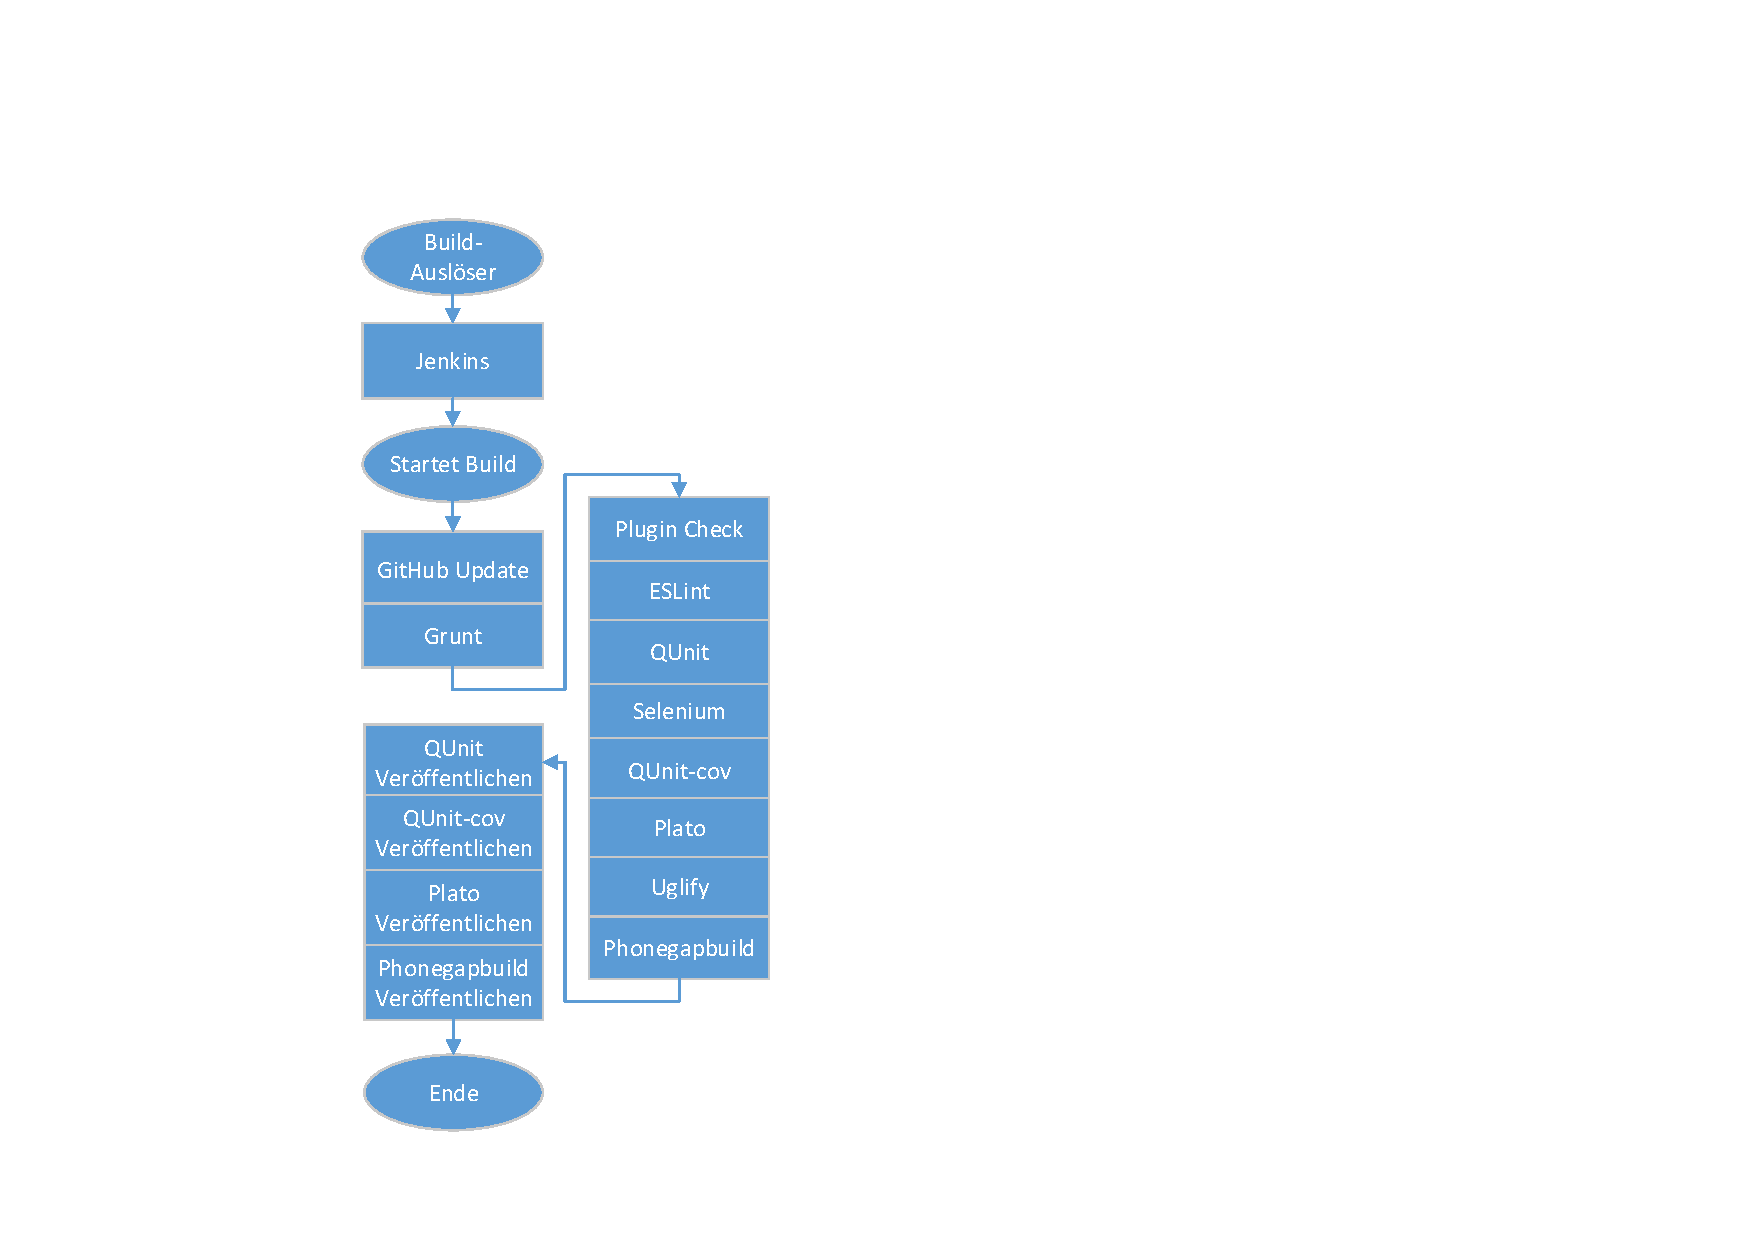
\includegraphics[trim = 45mm 15mm 20mm 35mm, scale=0.9]{ci-toolchain}
	\caption{Angepasste CI-Toolchain.}
	\label{fig:CI-Toolchain}
\end{figure}